\chapter{Related work}
\label{ch:related}


\section{Ms~Pac-Man}

\subsection{Overview}

\begin{wrapfigure}{r}{0.4\textwidth}
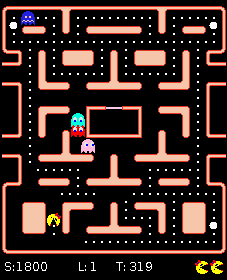
\includegraphics[width=\linewidth]{diagrams/pac-man}
\caption[The Ms Pac-Man game]{The Ms Pac-Man game: Ms Pac-Man is the yellow character, and is the one that the user controls.}
\label{fig:pac-man}
\end{wrapfigure}

The original Pac-Man was an arcade game developed by Toru Iwatani, a Japanese games designer working for Namco Company, in 1980~\citep{Samothrakis2011}.  It became hugely successful due to its wide appeal and a number of spin-offs were created.  One of these was Ms~Pac-Man, which was initially created unofficially before being sold to Midway Games, who distributed Namco games in North America.

The original game features a pizza-shaped protagonist ``Pac-Man'' which the player must direct around a maze consuming ``pills'' and occasionally fruit when it becomes available, whilst avoiding the four ghosts (``Pinky'', ``Inky'', ``Blinky'' and ``Clyde'') which attempt to eat Pac-Man.  If they succeed, Pac-Man loses a life.  There are four ``power pills'' in the maze: if Pac-Man eats one, all the ghosts turn blue and become edible.  Eating as many ghosts as possible in this state confers a significant advantage, as not only is the player rewarded with a number of points upon eating a ghost, the number of points on offer for a ghost doubles with each one eaten.  Starting at 200 for the first ghost, it increases to 400, 800, and 1600 for each consecutive ghost eaten whilst the same power pill is still active.  Thus, the total score available from a power pill is 3050 (50 for the power pill itself, and the sum of the scores mentioned above)---this is in contrast to only 10 points for each regular pill consumed.  Once all the pills in a maze have been cleared, the next level is reached.  Ghosts stay edible for decreasing amounts of time in each subsequent level, making it harder both to score points and to stay alive.

The original Pac-Man featured deterministic ghost behaviour and so it is possible to exploit known patterns of behaviour to learn how to play a given level in such a way that the maximum score for that level is always achieved.  However, Ms~Pac-Man features more sophisticated ghost behaviour which involves a level of non-determinism, making it much more difficult to play.  The other notable difference between the two games is that the latter has four levels instead of just one; there are other minor cosmetic differences such as the renaming of the orange ghost previously known as ``Clyde'' to ``Sue'', and the addition of a red bow and lipstick to the Pac-Man character.

\subsection{The Ms~Pac-Man environment}

Ms~Pac-Man is now more than thirty years old, a considerable time in the technology arena, and much more sophisticated games exist for the exponentially faster hardware available today; however, it remains useful to artificial intelligence research.  Much work has been done in creating game-playing agents for a wide range of games including chess, checkers, Go, and even Jeopardy, and these agents are often at least as good as human champions.  However, the task environment \cite[pp. 42--44]{RussellNorvig} of Ms~Pac-Man presents several interesting challenges not present in these games.

Unlike the games mentioned above, the Ms~Pac-Man environment is \emph{dynamic} rather than \emph{static}: whilst in chess the state of the game remains fixed between moves, the state in Ms~Pac-Man is continuously changing, even if the agent is not making any moves.  Additionally, rather than being afforded several minutes to deliberate, the agent must post a move relatively frequently (every 40~ms in the framework mentioned below).  Thus, the environment is also \emph{quasi-continuous} as opposed to being completely \emph{discrete} like board games.

Board games also tend overwhelmingly to be \emph{deterministic}, meaning that the results of a move can be completely and exactly determined by the agent.  In contrast, the Ms~Pac-Man environment is \emph{stochastic}: the ghosts incorporate random behaviour and therefore cannot be completely predicted.  Further complicating the problem of predicting the state of the game after a move is the fact that both Ms~Pac-Man and the ghosts make moves \emph{simultaneously} rather than taking turns as in the majority of board games.

However, the player does have knowledge of the whole game state available to them when making a decision, an attribute shared with traditional board games.  Similarly, all actions available to the player in a given state can be fully known and enumerated.

It can be seen that although Ms~Pac-Man is a seemingly simple, having a trivial objective and few rules, it is perhaps deceptively so, and certain aspects of the task environment greatly increase the complexity of developing an effective agent.  Accordingly, the performance of artificial agents falls somewhat short of the scores achieved by human players.

\subsection{Ms~Pac-Man frameworks}

The usefulness of Ms~Pac-Man to the field of artificial intelligence has previously been recognised and there exists a reasonable amount of research on the subject to date.  This has been encouraged by the creation of various frameworks and competitions to facilitate the development of artificial agents.  The original code is closed source and not designed to run on modern computers, and thus frameworks have had to be written to enable custom agent code to interface with the game.  Various authors~\citep{Lucas2005,Koza1992} have implemented their own simulated versions of the game, sometimes with quite different behaviour to the original game. \citet{Robles2009} also implemented their own version, as well as providing a framework which uses a screen capturing technique to allow the agent to extract information out of the original game running in an emulator.  They demonstrated that their simulator framework and the screen capture framework were roughly equivalent.

It is argued that exact equivalence to the real game is not important however, as the main motivation of such research is not necessarily to write an agent capable of playing the real game well (on its own, a goal of somewhat questionable utility); rather it is to write an agent capable of dealing with the kind of complexities inherent in a game such as Ms~Pac-Man.  As long as the simulated task environment is not significantly different to the real one as described above, the same benefits may be derived from the research.  It is nevertheless important to note that scores obtained by agents under different simulators cannot readily be compared.

The framework used in this work, the aforementioned simulator framework, was developed at the University of Essex~\citep{Robles2009} and used to host various competitions such as at the 2009 IEEE Conference on Computational Intelligence and Games (CIG 2012\footnote{\url{http://geneura.ugr.es/cig2012/}}) and at the IEEE World Congress on Computational Intelligence (WCCI 2012\footnote{\url{http://www.ieee-wcci2012.org/}}).  The framework is written in Java and closely replicates the original game, with a few notable exceptions:

\begin{itemize}
\item Ms~Pac-Man and the ghosts travel at the same speed, unless a power-pill is active, in which case Ms~Pac-Man can move faster than the ghosts.  Unlike the original, Ms~Pac-Man does not slow down when eating pills.
\item In the original, ghosts slow down in the ``tunnels'' at the side of the screen, providing an opportunity to put some distance between Ms~Pac-Man and a pursuing ghost.  This is not the case in the simulator.
\item The simulator does not include the bonus fruit.
\item The behaviour of the ghosts can be determined by any custom ghost controller class.  This is a significant difference which makes the task not only much harder, but arguably much more interesting, as tactics which are effective against one ghost ``team'' may not be effective against another.  The competitions generally feature user-submitted ghost teams as well as Ms~Pac-Man controllers and therefore it is not possible to know in advance what ghost teams the agent should be able to play against.  This point is the main reason behind this paper.
\end{itemize}

\section{Monte Carlo tree search}

\subsection{Introduction}

Traditional tree search algorithms have been successfully applied to numerous board games such as chess and checkers.  However, these algorithms have been found lacking in some areas, as they can be slow to run and require significant domain knowledge to produce effective agents.  More specifically, the \emph{evaluation function} which evaluates the strength of a particular game state has proven particularly difficult to write for many games.

One such game is Go \footnote{see \url{http://www.gobase.org} for an introduction}.  Chess has an 8~$\times$~8 board, and it is relatively easy to calculate from a given chess position which player has the upper hand by considering aspects such as material count and position.  On the other hand, the Go board (known as the \emph{Goban}) ranges from 9~$\times$~9 for beginners up to as large as 19~$\times$~19, and even experts disagree on the quality of given game states.  The technique of minimax search \cite[p. 165]{RussellNorvig} has proven very powerful for chess players, but the significantly higher branching factor of the game tree given by the larger board and the inability to write an effective \emph{evaluation function} for game states renders the technique of alpha-beta search ineffective for Go~\citep{Gelly2006}.

The Scrabble player \emph{Maven} was one of the first players to make use of simulated game play~\citep{Sheppard2002}.  The merits of different actions are evaluated by playing simulated games for each action, giving an insight into which move will prove to be the better choice as the game develops.  A similar technique has also been used for poker~\citep{Billings2002} and for backgammon~\citep{Tesauro1996}.  However, these players used uniform sampling of available actions or incorporated an unreliable heuristic, leading to much unnecessary simulation.  The UCT (``UCB applied to Trees'') algorithm~\citep{Kocsis2006} was developed in order to more intelligent chose actions to dedicate simulation time to; this effectively developed into the Monte Carlo tree search algorithm.

\subsection{Algorithm}

\begin{wrapfigure}{r}{0.4\textwidth}
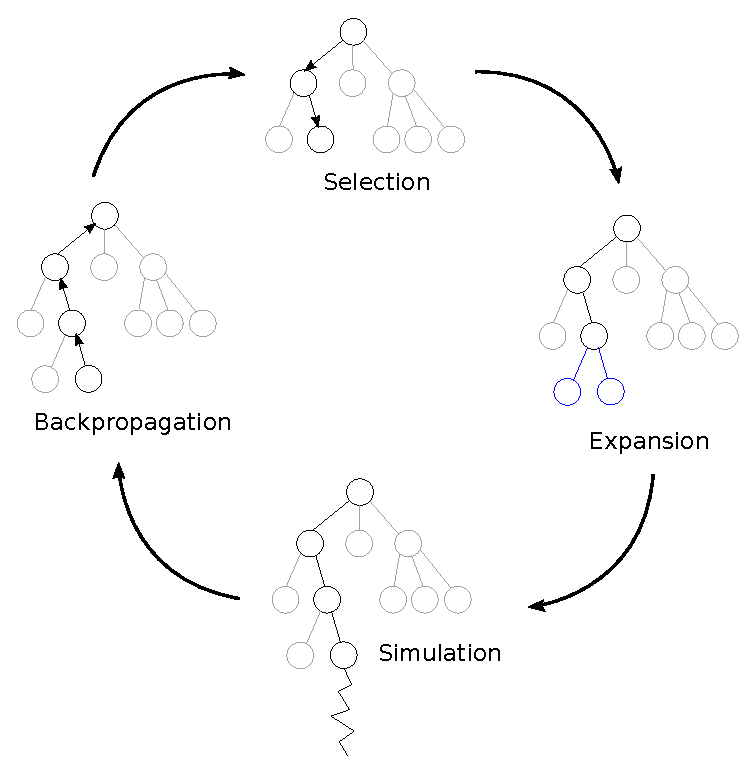
\includegraphics[width=\linewidth]{diagrams/mcts}
\caption{Monte Carlo tree search algorithm}
\label{fig:MCTS}
\end{wrapfigure}

Monte Carlo tree search (MCTS) is a best-first search technique in which many simulated games are run in order to build a tree of possible game states~\citep{Chaslot2008}.  Each node in the tree represents a game state after taking a given action, represented by the edge from the previous state to the new state.  The algorithm has the following four phases (illustrated in figure \ref{fig:MCTS}):

\textbf{Selection} ~Starting at the root node, the algorithm moves through the search tree by selecting a child of the current node according to some selection policy.  In order to avoid wasting time simulating games for poor moves, the policy must show a preference for choosing moves which have already demonstrated a good reward in previous simulations: this is known as \emph{exploitation}.  On the other hand, the policy must also choose nodes which have been sampled less, so that they may be further investigated: this is known as \emph{exploration}.  This \emph{exploitation versus exploration} dilemma is also seen in multi-armed bandit problems, for which various algorithms exist~\citep{Auer2002}.  The application of this type of algorithm to the selection phase of MCTS is what makes it useful over traditional Monte Carlo methods, as it dramatically decreases the search space.  The UCT algorithm~\citep{Kocsis2006} mentioned above is one of the most commonly-used algorithms for this.

\textbf{Expansion} ~Once a leaf node is reached, it may be expanded.  Expanding a node only once a certain sample count has been reached can produce better results.  If the node is expanded, one of its children should be chosen as the new leaf node: this can be a random decision, as the algorithm has no other information.

\textbf{Simulation} ~Also called \textbf{roll-out}, this phase involves running a simulated game from the game state represented by the leaf node arrived at.  In some of the earlier specifications of the algorithm, it was stated that the simulation should be continued until the end of the game~\citep{Chaslot2008}; however, it can also be run until some fixed point in the future, such as after a certain amount of moves.

\textbf{Backpropagation} ~After the simulated game has completed, the tree should be updated with the results.  This may be a simple win/loss ratio, but can be more complex.  For example, an n-player game may backpropagate a score for each player~\citep{Samothrakis2011}.

MCTS has been successfully applied to Go~\citep{Gelly2006} where it significantly improved upon the performance of existing players based on traditional tree search.  This is in part due to the efficient reduction in search space afforded by the UCT algorithm, and also because MCTS does not need an evaluation function.  Instead, random games are played from a game-state until the end of the game, and the score is backpropagated to the node.  MCTS has also been shown to be effective in nondeterministic games and those with imperfect information~\citep{Kocsis2006}.

As Ms Pac-Man has a high branching factor and is non-deterministic, MCTS is suited to the task.

\section{Previous Ms~Pac-Man agents}

One of the earliest known studies into Ms~Pac-Man was conducted by \citet{Koza1992}, using genetic programming \todo{Add details from book. D006.31 KOZ}.



\todo[inline]{Finish related work section}

\citet{Me2012} developed an agent using Monte Carlo tree search as part of an ensemble approach.  Prior to making a decision, any number of registered \emph{evaluators} are allowed to run to modify the results of the MCTS algorithm.  For example, a simple evalutor could spot moves in the game tree which eat power pills when there is already one active, and apply penalties to the scores of those nodes.  Thus, short- and long-range planning components augment the mid-range planning provided by the MCTS algorithm.

Although traditional MCTS utilises random playouts, the agent described in the paper uses more intelligent agents to control the playout behaviour, as this was found to have better results.  The paper explores two cases: the case where the model of the ghost behaviour used in the playouts matches the actual ghost controller being played against, and the case where the controllers differ.  In the former, three out of the four evaluator configurations considered were found to improve the score by a statistically significant amount, whilst the latter showed a significant improvement for only one evaluator.  Over all, the scores for the accurate model case were in the region of 50,000-60,000, a great deal more than the 10,000--15,000 achieved by the inaccurate model.

Clearly accurate domain knowledge improves the performance of the agent.  If the controller used during the playouts could adapt its behaviour based on observations of the controller being played against, one could reasonably expect the agent performance to steadily improve as the simulation model starts to more closely match the opponent controller.  This is the essence of this project.

\section{Machine learning}

\subsection{Introduction}

If an agent's performance on a given task improves as a result of observations made, it can be said to be learning \cite[p. 693]{RussellNorvig}.  It may not be clear why learning algorithms are needed; after all, surely the programmer should just program a system with the intended behaviour at the start.  However, this is not always possible.  For example, if one was to write a character recognition system, it would be impossible to foresee all of the possible slightly different forms a given character may take.  Furthermore, learning systems are good at responding to changes over time, that may not have been forseen by the original programmer.  Most importantly, sometimes it is impossible to imagine how to go about designing a particular algorithm---it is difficult to imagine how a manual face recognition algorithm might work for example.

\subsection{Neural networks}

Neural networks are modelled after the nervous system in humans and animals.  This is composed of (in humans, many billions of) cells called \emph{neurons}.  A wide variety of morphologies exist, but the majority of neurons consist of the same three parts: the \emph{dendrites}, highly branched structures which receive chemical signals from other nearby neurons; the \emph{cell body}, which contains the processes necessary for cell function; and the \emph{axon}, containing a ``trigger zone'' which generates electrical signals over the length of the axon if the input to the dendrites reaches a certain threshold.  The axon has \emph{axon terminals} at the opposite end to the dendrites and cell body; these transmit chemical messengers into the dendrites of connected neurons in response to an electrical impulse.  Neurons can be seen as \emph{integrators} as their output is a function of the inputs received from the many connected neurons \cite[p. 152]{Vander}.

Artificial neural networks also consist of large numbers of ``neurons''.  In general, these have a high-dimensional input vector and produce an output which is a non-linear \emph{activation} function (often a sigmoid function) of the input vector and some weights vector \cite[p. 1]{Annema1995}.  It can readily be appreciated how this is analogous to the biological system: the input vector represents the many incoming connections to the dendrites, while the ``trigger zone'' and axon terminals are represented by the activation function and its output.

Each element of the input vector is multiplied by a corresponding element in the weights vector before being summed and used as the input to the activation function; thus, the weights vector controls how much each input affects the output of the neuron.  The weights are adjusted in a \emph{training phase}: by using a large number of training examples where the output expected of the neuron is known, the weights can be iteratively modified according to a learning rule which seeks to minimise the error between the actual output of the neuron and the expected output for each training example \cite[p. 1]{Annema1995}.  This is a form of \emph{supervised learning} \cite[p. 695]{RussellNorvig}.

Although the exact mechanism of learning in the brain is not fully understood, it is thought to operate along similar lines.  In the \emph{long-term potentiation} model, the connections between neurons (called \emph{synapses}) increase in effectiveness when heavily used \cite[p. 271]{Vander}, which is similar in function to the weights which govern the connections between artificial neurons changing value.

\todo[inline]{Add something from Rumelhart et al (D153.4 PAR)}

The type of artificial neural network used in this work is the two-layer feed-forward network \cite[p. 4]{Aleksander1995}.  This consists of a layer of neurons called the \emph{hidden layer}, which computes some internal representation of the inputs \cite[p. 135]{Aleksander1995}, and a connected \emph{output layer}, which computes the final result of the neural network as a function of the output from the hidden layer.  The term ``feed-forward'' refers to the fact that the input is passed first to the hidden layer, and then fed forward to the output layer.  It has been shown that such a network is capable of approximating any function \cite[p. 10]{Annema1995}.

\todo[inline]{Maybe add Kolmogrov's theorem (p. 10 of Annema) and comment from p. 135 of Aleksander et al}

The use of a hidden layer introduces a problem---the expected output for the hidden layer is not known, and so some method must exist for propagating the errors from the output layer in order to train the weights in the hidden layer.  The algorithm used for this purpose in this work is the backpropagation algorithm \cite[pp. 134--149]{Aleksander1995}, which will be discussed in more detail in the implementation section.
